\section{Analytic Functions}

\begin{definition}
    We say a complex valued function $f:U \xrightarrow{} \C$ on an open domain $U$
    of $\C$ is  \textbf{analytic} at a point $z_0 \in U$ if there exists a
    convergent power series $\sum{a_n(z-z_0)^n}$ with radius of convergence
    $r>0$ for which
    \begin{equation*}
        f(z)=\sum{a_n(z-z_0)^n}
    \end{equation*}
    and we call $\sum{a_n(z-z_0)^n}$ the \textbf{power series expansion} of $f$
    at $z_0$. We say that $f$ is  \textbf{analytic} on $U$ if it is analytic at
    every point of $U$. If $S \subseteq \C$, we say that $f$ is \textbf{analytic} on
    $S$ if $f$ is the restriction of an analytic function on some open set
    containing $S$. If $a_0=0$ in the power series, we call $z_0$ a
    \textbf{zero} of $f$ if  $f(z_0)=0$.
\end{definition}

\begin{theorem}\label{2.4.1}
    Let $f$ and  $g$ be analytic functions on an open domain $U$ of $\C$. Then
    $f+g$, and $fg$ are analytic on  $U$.
\end{theorem}
\begin{proof}
    Let $f(z)=\sum{a_n(z-z_0)}$, $g(z)=\sum{b_n(z-z_0)^n}$ for any $z_0 \in U$.
    Then $(f+g)(z)=\sum{(a_n+b_n)(z-z_0)^n}$ and $(fg)(z)=\sum{c_n(z-z_0)^n}$.
    Since the power series expansions of $f$ and  $g$ at  $z_0$ are convergent,
    the power series expansions of $f+g$ and  $fg$ at  $z_0$ are also convergent
    by theorem \ref{2.3.1}. Therefore $f+g$ and  $fg$ are analytic.
\end{proof}
\begin{corollary}
    $\frac{f}{g}$ is analytic on $U$ provided that $g(z) \neq 0$ for all $z \in
    U$.
\end{corollary}

\begin{theorem}\label{2.4.2}
    Let $U,V$ be open sets in $\C$. If $g:U \xrightarrow{} \C$ and $f:V
    \xrightarrow{} \C$ are analytic functions on $U$ and  $V$, respectively, and
     $g(U) \subseteq V$, then $f \circ g:U \xrightarrow{} \C$ is analytic on
     $U$.
\end{theorem}
\begin{proof}
    Since compositions of convergent power series are convergent, this makes $f
    \circ g$ convergent.
\end{proof}

\begin{theorem}\label{2.4.3}
    Let $f(z)=\sum{a_nz^n}$ be a convergent power series with radius of
    convergence $r>0$. Then  $f$ is analytic on the open ball $B(0,r)$ as a
    complex valued function.
\end{theorem}
\begin{proof}
    Choose $z_0 \in B(0,r)$ so that $|z_0|<r$ and let $s>0$ such that
    $|z_0|+s<r$. Then $f$ can be represented as a power series at $z_0$ which
    converges absolutely on an open ball $B(z_0,s)$ (see figure \ref{figure_2.1}).
    Writing $z=z_0+(z_-z_0)$ so that $z^n=(z_0+(z-z_0))^n$, we have that
    \begin{equation*}
        f(z)=\sum_{n=0}^\infty{a_n\sum_{k=0}^n{{n \choose k}z_0^{n-k}(z-z_0)^k}}
    \end{equation*}
    Now, if $|z-z_0|<s$, then $|z_0|+|z-z_0|<r$ and the series
    \begin{equation*}
        \sum_{n=0}^\infty{|a_n|(|z_0|+|z-z_0|)^n}
    \end{equation*}
    converges. Interchanging the order of summation gives us the required
    result.
\end{proof}

\begin{figure}[h]
    \centering
    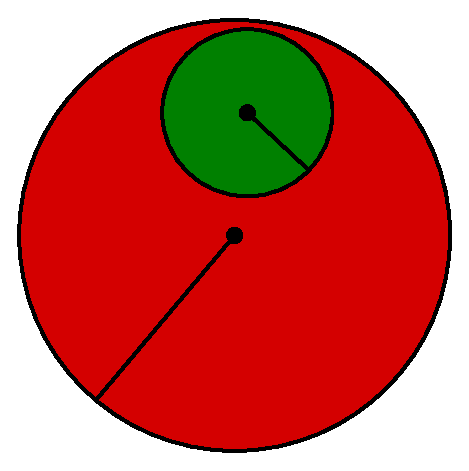
\includegraphics[scale=0.5]{Figures/Chapter2/analytic_ball.eps}
    \caption{}
    \label{figure_2.1}
\end{figure}

\begin{example}\label{example_2.8}
    \begin{enumerate}
        \item[(1)] Consider $f(z)=\frac{z^2}{z+2}$ and $z_0=1$. Writing
            $z=1+(z-1)$, and $z+2=3+(z-1)$, then $z^2=1+2(z-1)+(z-1)^2$,
            $z+2=3(1+\frac{1}{3}(z-1))$, and
            \begin{equation*}
                \frac{1}{z+2}=\frac{1}{3}(1-\frac{1}{3}(z-1)+\frac{1}{3^2}(z-1)^2)
                -\frac{1}{3^3}(z-1)^3+\dots
            \end{equation*}
            Thus, we get the power series expansion of $f$ at $z_0=1$ to be
            \begin{align*}
                \frac{z^2}{z+2} &=  (1+2(z-1)+(z-1)^2+\dots)
                (\frac{1}{3}(1-\frac{1}{3}(z-1)+\frac{1}{3^2}(z-1)^2)
                -\frac{1}{3^3}(z-1)^3+\dots) \\
                                &= \frac{1}{3}(1+\frac{5}{3}(z-1)+
                                (\frac{1}{3}+\frac{1}{3^2})(z-1)^2)+
                                (\frac{1}{3}+\frac{1}{3^2}+\frac{1}{3^3})(z-1)^3+
                                \dots   \\
            \end{align*}
    \end{enumerate}
\end{example}
